\documentclass[conference]{IEEEtran}
\IEEEoverridecommandlockouts

\usepackage{cite}
\usepackage{amsmath,amssymb,amsfonts}
\usepackage{algorithmic}
\usepackage{graphicx}
\usepackage{textcomp}
\usepackage{xcolor}
\usepackage{booktabs}
\usepackage{url}

\begin{document}

\title{Deadline-Aware Adaptive Vision Transformer Inference for Soft Real-Time Edge Workloads}

\author{\IEEEauthorblockN{Anonymous Authors}
\IEEEauthorblockA{\textit{Real-Time Systems Research Laboratory} \\
Draft Manuscript Prepared for Peer Review}
}

\maketitle

\begin{abstract}
Vision Transformers (ViTs) deliver superior accuracy for autonomous perception, but their quadratic computational complexity and variable execution times create significant challenges for latency-critical cyber-physical systems. While token pruning techniques such as EViT reduce arithmetic operations, algorithmic complexity reductions alone do not guarantee deadline satisfaction on physical graphics hardware. In this paper, we investigate deadline-aware adaptive vision transformer inference for soft real-time edge workloads. We propose an integrated real-time scheduling framework that combines empirical hardware latency profiling, dynamic token-pruning model selection, priority-driven queuing, and lightweight admission control. Fine-tuning DeiT-Small and three EViT configurations ($k \in \{0.9, 0.7, 0.5\}$) on the complete BDD100K driving scene dataset (99,483 valid images across six scene classes), we demonstrate that pruning up to 50\% of tokens reduces multiply-accumulate operations (MACs) by 49.8\% with only a 0.80 percentage-point drop in top-1 accuracy (77.64\% to 76.84\%). Profiled on a dedicated NVIDIA GeForce RTX 4060 GPU using static CUDA Graphs, token pruning yields a 30.7\% reduction in median inference latency (3.231~ms to 2.236~ms) and an empirical p95 execution time of 2.806~ms. Across a canonical discrete-event simulation suite of 70 workload-policy configurations (covering periodic, jittered, bursty, and overload arrivals), our proposed adaptive earliest-deadline-first policy with admission control improves the on-time completion ratio by up to +73 percentage points over static baselines under severe stress (79\% vs.\ 6\% in high jittered traffic; 76\% vs.\ 7\% under high periodic load). Physical hardware trace replay over 100 unique canonical test images corroborates the simulation with makespan agreement within $-0.57\%$ to $-0.07\%$. Our findings establish that pairing dynamic token pruning with admission control and deadline-aware dispatching effectively mitigates transient queuing delays in soft real-time edge vision systems.
\end{abstract}

\begin{IEEEkeywords}
Real-Time Systems, Vision Transformers, Token Pruning, EViT, Earliest Deadline First, Admission Control, BDD100K, CUDA Graphs, Edge Computing.
\end{IEEEkeywords}

\section{Introduction}

Autonomous mobile platforms, including self-driving vehicles, uncrewed aerial vehicles, and robotic manipulators, rely on vision sensors to perceive dynamic environments \cite{grigorescu2020survey, yu2020bdd100k}. In these cyber-physical systems, visual perception tasks (such as driving scene classification, obstacle detection, and trajectory forecasting) are governed by stringent timing constraints. An inference result that arrives after its deadline is stale and can jeopardize platform safety \cite{buttazzo2011hard}.

Recently, Vision Transformers (ViTs) \cite{dosovitskiy2021image, touvron2021training} have emerged as a dominant architecture for visual perception, demonstrating remarkable robustness against domain shifts and environmental perturbations. Nevertheless, deploying ViTs in real-time edge systems remains notoriously challenging. The core multi-head self-attention (MHSA) mechanism exhibits quadratic complexity with respect to the sequence length $N$ ($O(N^2)$), consuming extensive GPU memory bandwidth and introducing tail-latency variability.

To accelerate vision transformers, token pruning and token reorganization techniques have been proposed \cite{liang2022not, rao2021dynamicvit, kong2022spvit}. Notably, the Efficient Vision Transformer (EViT) \cite{liang2022not} identifies inattentive image patches and reorganizes them into a single summary token, significantly reducing theoretical multiply-accumulate operations (MACs). However, in real-time computing, computational reduction does not inherently imply deadline satisfaction \cite{buttazzo2011hard}. A faster model deployed under an oblivious First-In, First-Out (FIFO) queue can still miss deadlines during bursty traffic, while static deployment of an aggressive pruning variant unnecessarily degrades perception accuracy during low-load intervals.

\begin{figure*}[t]
\centering
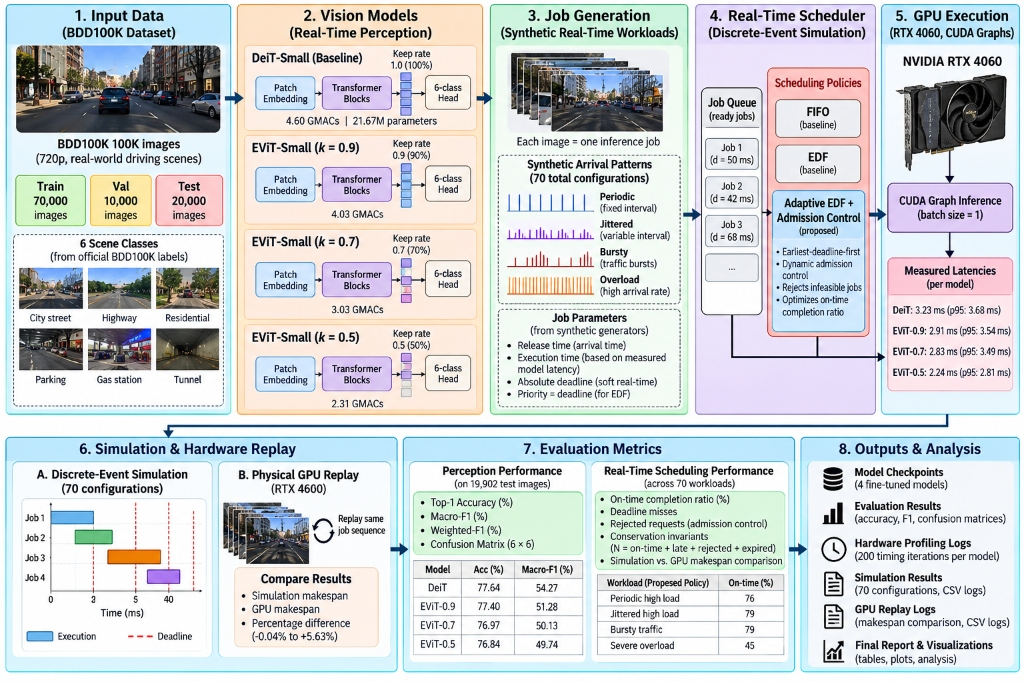
\includegraphics[width=0.95\linewidth]{figures/system_architecture.jpg}
\caption{End-to-end architecture of the deadline-aware adaptive vision transformer inference system: from BDD100K driving scene dataset partitioning and multi-configuration EViT perception models to synthetic workload generation, discrete-event scheduling simulation, physical CUDA Graph replay on an NVIDIA RTX 4060 GPU, and comprehensive metric evaluation.}
\label{fig:arch}
\end{figure*}

This paper addresses the central research question: \textit{Can adaptive selection among full and token-pruned vision transformers, orchestrated by deadline-aware scheduling and admission control, significantly increase the fraction of offered requests completed before their deadlines under variable edge workloads?}

To investigate this question, we develop an end-to-end real-time vision inference pipeline, depicted in Fig.~\ref{fig:arch}. Our work makes the following contributions:
\begin{enumerate}
    \item \textbf{Perception-Accuracy Trade-off Characterization:} We fine-tune and evaluate DeiT-Small \cite{touvron2021training} and three EViT variants ($k \in \{0.9, 0.7, 0.5\}$) on the full 100,000-image BDD100K driving scene dataset \cite{yu2020bdd100k} (99,483 valid records across six scene classes), quantifying the trade-off between token keep rate, arithmetic complexity, top-1 accuracy, and macro-F1 across 19,902 held-out test images.
    \item \textbf{Deterministic GPU Latency Profiling:} We capture static CUDA Graphs \cite{nvidia2023cudagraphs} on a dedicated NVIDIA GeForce RTX 4060 Laptop GPU at batch size 1 (FP32), demonstrating a 4.0x--10.9x speedup over eager PyTorch and characterizing empirical mean, median, p95, and p99 execution distributions.
    \item \textbf{Controlled Synthetic Workload Suite:} We implement a parameterized synthetic workload trace generator modeling periodic, jittered, bursty, and overload traffic across four traffic intensities ($\rho \in \{0.50, 0.85, 1.15, 1.50\}$) and tight, moderate, and loose deadline constraints.
    \item \textbf{Deadline-Aware Real-Time Scheduler:} We formulate a priority-driven scheduling architecture supporting FIFO and Earliest Deadline First (EDF) queuing, monotonic counter tie-breaking, slack-aware adaptive model selection with quality thresholds, and an $O(|Q|)$ queue-tail admission control heuristic.
    \item \textbf{Discrete-Event Simulation and Hardware Validation:} We evaluate 70 workload-policy configurations in discrete-event simulation, verify four fundamental real-time request conservation equations with zero errors, and validate the simulation against live physical GPU trace replay over 100 unique canonical test images, achieving makespan agreement within $-0.57\%$ to $-0.07\%$.
\end{enumerate}

\section{Related Work}

\subsection{Efficient Vision Transformers \& Token Pruning}
Following the introduction of ViT \cite{dosovitskiy2021image} and data-efficient distillation \cite{touvron2021training}, substantial research has targeted transformer efficiency. DynamicViT \cite{rao2021dynamicvit} trained lightweight prediction modules to drop uninformative tokens hierarchically. Liang et al.\ \cite{liang2022not} proposed EViT, which identifies top-$k$ attentive tokens based on the \texttt{[CLS]} token attention map, fuses inattentive tokens into a single representation token, and achieves significant throughput gains without auxiliary routing networks. SPViT \cite{kong2022spvit} integrated latency-aware loss formulations into soft token pruning. While these works demonstrate reduced FLOPs on ImageNet benchmarks, they do not address temporal deadline constraints, priority queuing, or dynamic workload bursts in cyber-physical edge systems.

\subsection{Real-Time Deep Learning Inference Scheduling}
Classical real-time scheduling theory provides predictable execution bounds for periodic and aperiodic tasks \cite{buttazzo2011hard}. Applying these principles to deep neural network (DNN) serving has gained traction. DeepRT \cite{zhang2021deeprt} developed a soft real-time scheduler for computer vision applications on edge devices, coordinating preemptive CPU-GPU execution. DART \cite{le2022dart} investigated dynamic resource-aware scheduling for multi-task vision workloads. Other approaches dynamically adapt model architectures via early-exit branches \cite{teerapittayanon2016branchynet} or resolution scaling \cite{yang2020resolution}. However, most prior real-time schedulers evaluate convolutional networks or rely on synthetic execution-time assumptions rather than evaluating multi-stage token-pruning vision transformers under static CUDA Graph execution on physical GPU hardware.

\section{System Model and Problem Formulation}

\subsection{Hardware Platform \& Execution Semantics}
We consider a dedicated edge computing platform equipped with a host CPU and an NVIDIA GeForce RTX 4060 Laptop GPU (AD107M architecture, 3,072 CUDA cores, 8~GB GDDR6 memory, 115W TGP). In real-time computer vision, running inference via standard eager-mode frameworks incurs substantial host-side latency taxes (Python interpreter overhead, driver launches, and asynchronous kernel queueing), introducing up to 15--20~ms of jitter.

To enforce predictable execution, all vision transformer models are instantiated as static \textbf{CUDA Graphs} \cite{nvidia2023cudagraphs}. During offline initialization, the model's forward execution graph is captured into static GPU memory at batch size 1 (FP32). At runtime, invoking the graph bypasses CPU-side kernel dispatch entirely, dispatching all operations directly on the GPU command processor. Execution is \textbf{non-preemptive}: once a forward pass begins on the GPU, it runs to completion without interruption.

\subsection{Real-Time Request Model}
The real-time vision system processes a sequence of inference requests $\mathcal{R} = \{r_0, r_1, \dots, r_{N-1}\}$:
\begin{equation}
r_i = (A_i, \, D_{\text{rel}, i}, \, D_{\text{abs}, i}, \, \mathbf{x}_i, \, y_i)
\end{equation}
where:
\begin{itemize}
    \item $A_i \in \mathbb{R}_{\ge 0}$ is the release (arrival) timestamp in milliseconds (ms), with $A_0 = 0.0$~ms.
    \item $D_{\text{rel}, i} \in \mathbb{R}_{> 0}$ is the relative deadline budget in milliseconds.
    \item $D_{\text{abs}, i} = \text{round}(A_i + D_{\text{rel}, i}, \, 4)$ is the absolute deadline timestamp in milliseconds.
    \item $\mathbf{x}_i \in \mathbb{R}^{3 \times 224 \times 224}$ is the input driving scene frame.
    \item $y_i \in \{0, \dots, 5\}$ is the ground-truth driving scene label.
\end{itemize}

\subsection{Candidate Model Suite}
The system maintains a resident pool of $M=4$ fine-tuned vision models $\mathcal{M} = \{m_0, m_1, m_2, m_3\}$, where $m_0$ is the unpruned baseline (\texttt{deit\_small\_baseline}) and $m_1, m_2, m_3$ represent EViT variants with decreasing keep rates ($k \in \{0.9, 0.7, 0.5\}$). Each candidate model $m \in \mathcal{M}$ is characterized by:
\begin{enumerate}
    \item Validation accuracy $\text{Acc}_{\text{val}}(m) \in [0, 100]\%$.
    \item Empirical p95 latency estimate $C_m = \text{Lat}_{p95}(m)$ in milliseconds.
\end{enumerate}

\subsection{Objective and Performance Metrics}
The system operates under \textbf{firm real-time constraints}: an inference result completed after its absolute deadline provides zero utility. If a request cannot complete before $D_{\text{abs}, i}$, it should be dropped or rejected to preserve GPU cycles for feasible requests.

Let $N_{\text{offered}} = |\mathcal{R}|$ denote the total requests offered to the system. The primary Quality-of-Service (QoS) objective is to maximize the \textbf{on-time completion ratio} over offered requests:
\begin{equation}
\text{Maximize} \quad \text{OnTimeRatio} = \frac{N_{\text{completed\_on\_time}}}{N_{\text{offered}}}
\end{equation}
subject to the constraint that for all completed requests:
\begin{equation}
t_{\text{finish}, i} \le D_{\text{abs}, i} + \epsilon_{\text{tol}}
\end{equation}
where $\epsilon_{\text{tol}} = 10^{-6}$~ms accommodates floating-point precision limits. Secondary objectives include minimizing request waiting time and maximizing delivered classification accuracy among completed requests.

\section{Dataset and Perception Models}

\subsection{The BDD100K Driving Scene Dataset}
We evaluate our system on the Berkeley DeepDrive (BDD100K) dataset \cite{yu2020bdd100k}, capturing diverse autonomous driving conditions. While the complete image archive comprises 100,000 JPEG images ($1280 \times 720$ resolution), our audit revealed that 517 records lack valid scene annotations (\texttt{undefined}). Filtering these records yields \textbf{99,483 valid driving scene records}, partitioned into canonical splits:
\begin{itemize}
    \item \textbf{Training Split:} 69,634 images.
    \item \textbf{Validation Split:} 9,947 images.
    \item \textbf{Test Split:} 19,902 images.
\end{itemize}

The dataset exhibits natural class imbalance across the six scene categories: City street (60.91\%), Highway (24.08\%), Residential (11.75\%), Parking lot (1.93\%), Gas stations (0.97\%), and Tunnel (0.35\%). Image filenames are strictly disjoint across all splits; sequence prefix checking identified a single shared prefix between training and validation sequences, while the 19,902-image test split is completely isolated.

\begin{figure}[t]
\centering
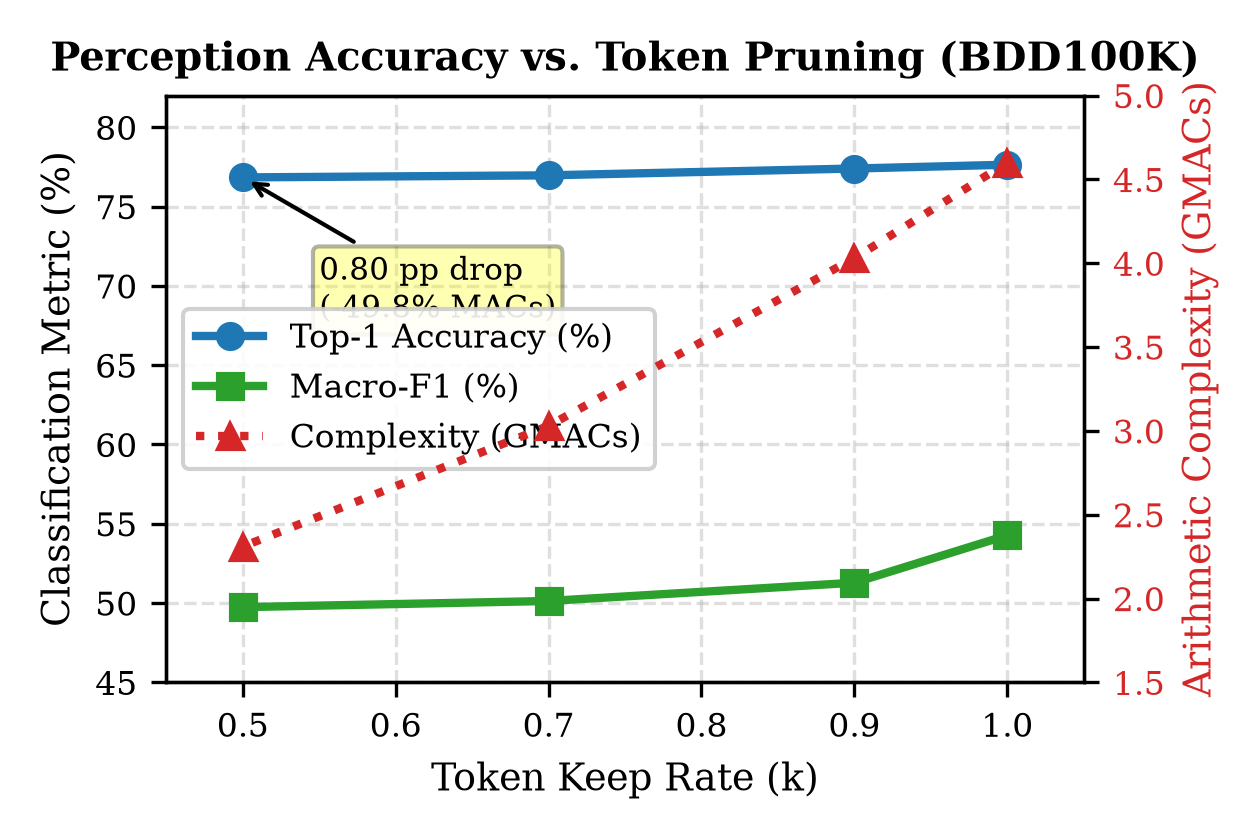
\includegraphics[width=\columnwidth]{figures/fig2_perception_tradeoff.png}
\caption{Perception accuracy (Top-1 and Macro-F1) versus token keep rate $k$ and arithmetic complexity (GMACs) on the 19,902-image BDD100K test split.}
\label{fig:perception_tradeoff}
\end{figure}

\begin{table}[t]
\centering
\caption{Perception Accuracy and Complexity on Held-Out BDD100K Test Set (19,902 Images)}
\label{tab:models}
\resizebox{\columnwidth}{!}{%
\begin{tabular}{lcccccc}
\toprule
Model Configuration & Keep ($k$) & MACs & Top-1 & Macro-F1 & W-F1 & Correct \\
\midrule
\texttt{deit\_small\_baseline} & 1.00 & 4.60~G & 77.64\% & 54.27\% & 77.20\% & 15,452 \\
\texttt{evit\_small\_k09\_fuse} & 0.90 & 4.03~G & 77.40\% & 51.28\% & 76.23\% & 15,404 \\
\texttt{evit\_small\_k07\_fuse} & 0.70 & 3.03~G & 76.97\% & 50.13\% & 75.71\% & 15,318 \\
\texttt{evit\_small\_k05\_fuse} & 0.50 & 2.31~G & 76.84\% & 49.74\% & 75.68\% & 15,292 \\
\bottomrule
\end{tabular}%
}
\end{table}

\subsection{Vision Transformer Architecture \& Token Pruning}
We adopt DeiT-Small \cite{touvron2021training} as our foundational backbone ($D = 384$ embedding dimension, $L = 12$ transformer blocks, $H = 6$ attention heads, patch size $P = 16$). Standard $224 \times 224$ input images produce a sequence of $14 \times 14 = 196$ visual tokens plus one prepended \texttt{[CLS]} token. The classification head is a linear projection ($384 \to 6$) matching the six driving scene categories, resulting in exactly \textbf{21,668,022 parameters} ($\approx 21.67$M) across all variants.

Following Liang et al.\ \cite{liang2022not}, EViT prunes tokens dynamically at layers 3, 6, and 9. At each pruning layer, attention scores between the \texttt{[CLS]} token and all patch tokens are computed:
\begin{equation}
\mathbf{s} = \text{Softmax}\left(\frac{\mathbf{q}_{\text{CLS}} \mathbf{K}^T}{\sqrt{d_k}}\right)
\end{equation}
The top-$\lfloor k \cdot N_l \rfloor$ tokens are retained as unperturbed patch tokens. The remaining $(1-k)N_l$ inattentive tokens are fused via weighted average into a single summary token:
\begin{equation}
\mathbf{t}_{\text{fuse}} = \sum_{j \in \mathcal{U}} \frac{\mathbf{s}_j}{\sum_{m \in \mathcal{U}} \mathbf{s}_m} \mathbf{x}_j
\end{equation}
where $\mathcal{U}$ denotes the index set of inattentive tokens. This summary token is concatenated back into the sequence, preserving global scene context while dropping spatial computation paths.

\subsection{Perception Accuracy on Full BDD100K Test Set}
All models were fine-tuned on the 69,634 training images using AdamW (batch size 64, learning rate $5 \times 10^{-5}$, cosine schedule, 5 epochs). Checkpoints were selected strictly on validation accuracy. Test evaluation was performed on the 19,902 held-out test frames.

As illustrated in Fig.~\ref{fig:perception_tradeoff} and detailed in Table~\ref{tab:models}, EViT exhibits graceful accuracy degradation:
\begin{itemize}
    \item Pruning 10\% of tokens ($k=0.9$) saves 0.57 GMACs ($-12.4\%$) with only a 0.24 percentage-point (pp) drop in top-1 accuracy.
    \item Pruning 50\% of tokens ($k=0.5$) cuts arithmetic complexity by nearly half ($-49.8\%$ MACs) while retaining \textbf{76.84\% top-1 accuracy}, representing an absolute decline of only 0.80~pp (1.03\% relative loss).
    \item Macro-F1 scores (49.74\%--54.27\%) are lower than top-1 accuracy due to natural class imbalance, as false negatives on rare categories (tunnel, gas station) heavily penalize unweighted class averages.
\end{itemize}

\begin{figure*}[t]
\centering
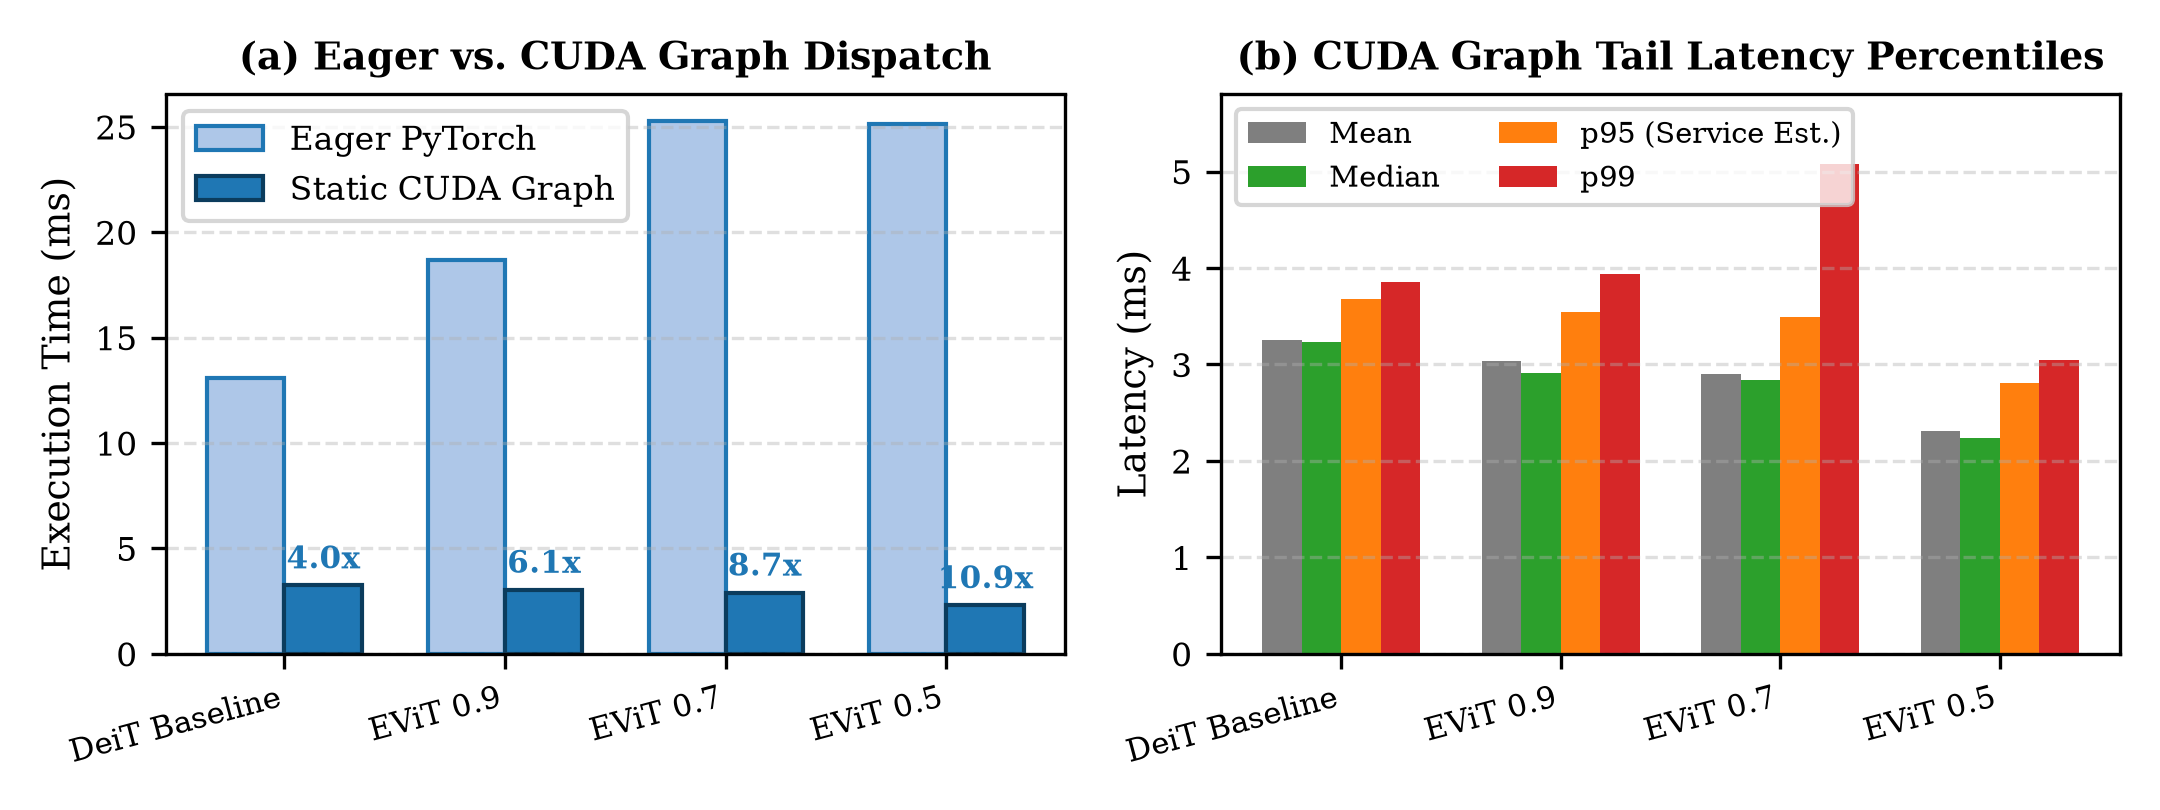
\includegraphics[width=0.92\linewidth]{figures/fig3_gpu_latency_profiles.png}
\caption{Physical GPU latency profiling on NVIDIA RTX 4060: (a) Eager PyTorch vs.\ static CUDA Graph execution, illustrating the 4.0x--10.9x speedup from kernel launch elimination; (b) Empirical tail latency percentiles (Mean, Median, p95, p99) across token pruning configurations.}
\label{fig:latency_profiles}
\end{figure*}

\section{GPU Latency Profiling}

\subsection{Benchmarking Methodology}
Physical profiling was conducted on the dedicated NVIDIA GeForce RTX 4060 Laptop GPU in FP32 precision at batch size 1. Following 50 warmup iterations, execution times were captured across 200 consecutive iterations on the CUDA timeline using \texttt{torch.cuda.Event(enable\_timing=True)}.

\begin{table}[t]
\centering
\caption{Physical GPU Latency Profiles on RTX 4060 (FP32, Batch Size 1, Static CUDA Graphs)}
\label{tab:latencies}
\resizebox{\columnwidth}{!}{%
\begin{tabular}{lcccccc}
\toprule
Model Configuration & Keep ($k$) & Mean & Med. & \textbf{p95 ($C_m$)} & p99 & FPS \\
\midrule
\texttt{deit\_small\_baseline} & 1.00 & 3.250~ms & 3.231~ms & \textbf{3.683~ms} & 3.859~ms & 417.1 \\
\texttt{evit\_small\_k09\_fuse} & 0.90 & 3.039~ms & 2.914~ms & \textbf{3.543~ms} & 3.939~ms & 469.0 \\
\texttt{evit\_small\_k07\_fuse} & 0.70 & 2.905~ms & 2.834~ms & \textbf{3.491~ms} & 5.080~ms & 557.3 \\
\texttt{evit\_small\_k05\_fuse} & 0.50 & 2.308~ms & 2.236~ms & \textbf{2.806~ms} & 3.047~ms & 610.4 \\
\bottomrule
\end{tabular}%
}
\end{table}

\subsection{Profiling Insights \& Non-WCET Classification}
\begin{enumerate}
    \item \textbf{CUDA Graph Dispatch Elimination:} Eager PyTorch on Windows exhibits 13.11~ms to 25.27~ms mean latency. As shown in Fig.~\ref{fig:latency_profiles}(a), static CUDA Graphs eliminate host kernel launch bottlenecks, accelerating DeiT baseline by \textbf{4.0x} (13.11~ms $\to$ 3.25~ms) and EViT-0.5 by \textbf{10.9x} (25.12~ms $\to$ 2.31~ms).
    \item \textbf{Monotonic Latency Reduction:} As summarized in Table~\ref{tab:latencies} and Fig.~\ref{fig:latency_profiles}(b), pruning tokens from $k=1.0$ to $k=0.5$ monotonically reduces median execution latency from 3.231~ms to 2.236~ms (\textbf{30.7\% latency reduction}) and scales throughput from 417.1 FPS to \textbf{610.4 FPS} (+46.3\%).
    \item \textbf{Statistical Tail Classification:} \textit{The reported p95 and p99 values are empirical statistical percentiles from measured sample distributions and are NOT formal deterministic Worst-Case Execution Times (WCET).} In our discrete-event simulator, the empirical p95 latency is used as a deterministic service-time estimate ($C_m = \text{Lat}_{p95}(m)$).
\end{enumerate}

\begin{figure*}[t]
\centering
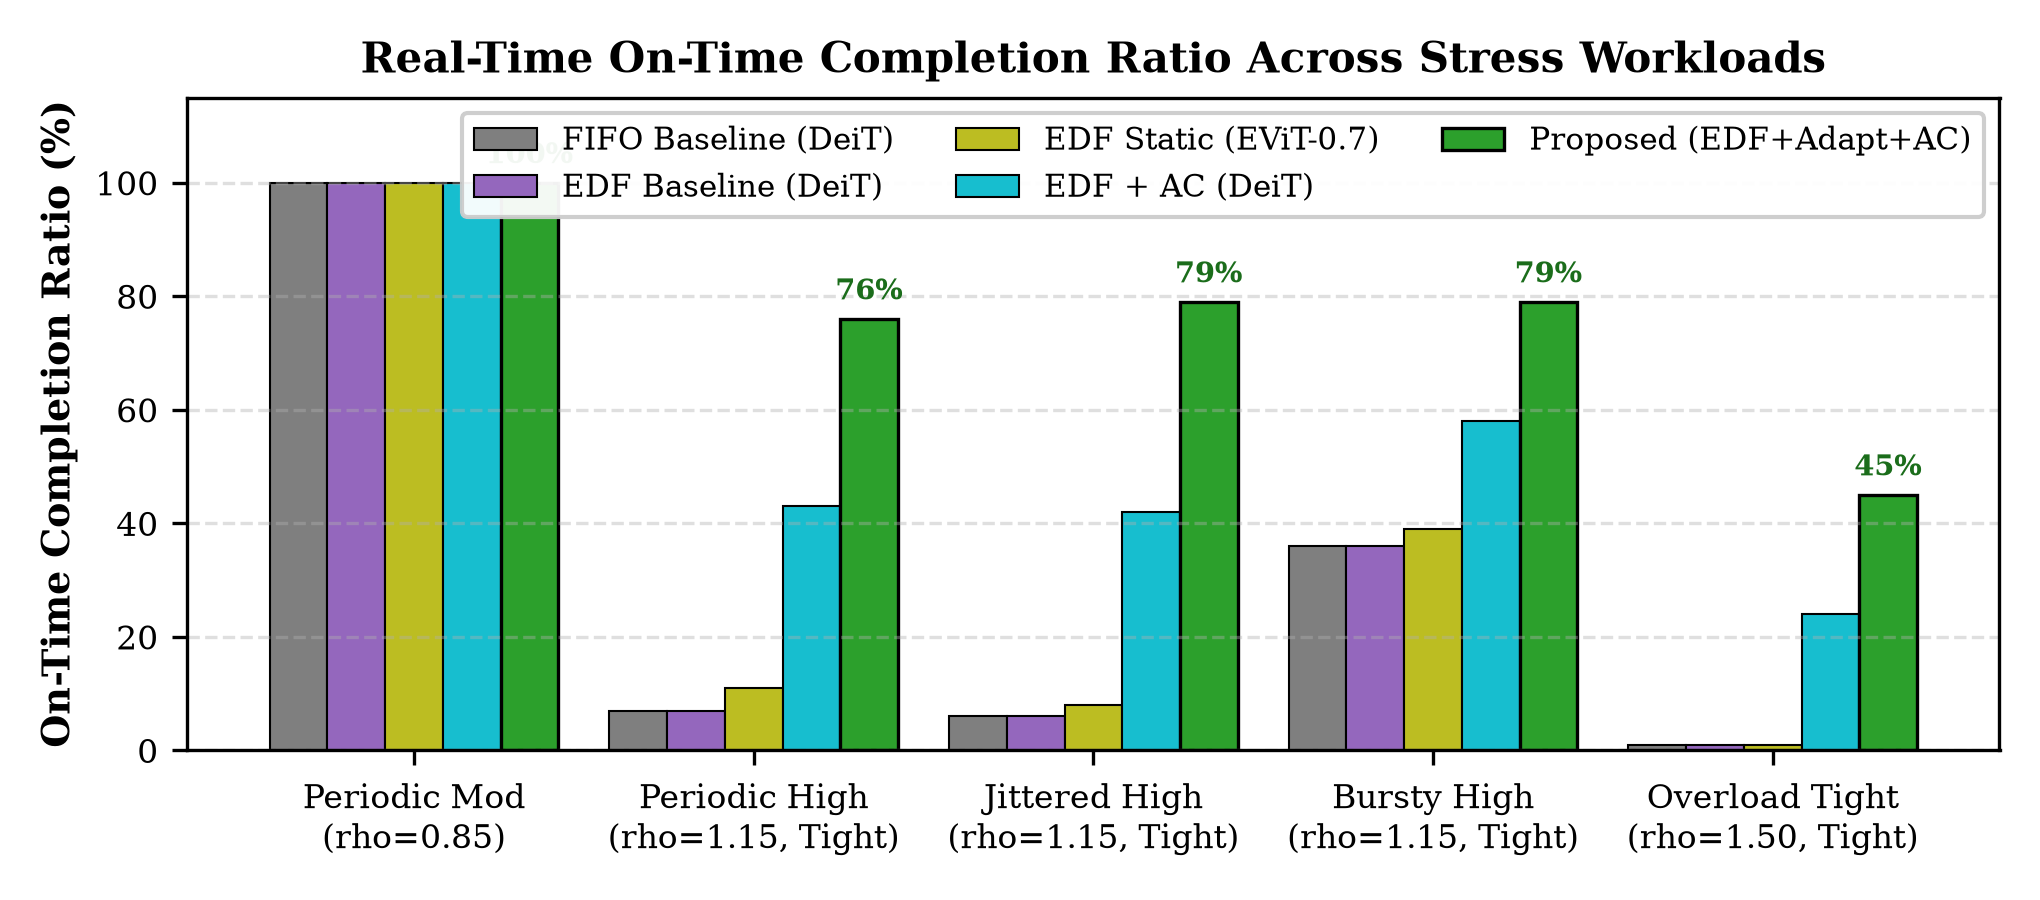
\includegraphics[width=0.88\linewidth]{figures/fig4_scheduling_ontime_comparison.png}
\caption{Real-time on-time completion ratio comparison across representative stress workloads for baseline and proposed policies, showing the +69~pp and +73~pp gains under heavy traffic saturation.}
\label{fig:ontime_comparison}
\end{figure*}

\section{Workload Generation}

To evaluate scheduling resilience under reproducible stress conditions, we construct a parameterized synthetic workload trace generator.

\begin{table}[t]
\centering
\caption{Synthetic Workload Suite Parameters ($N=100$ Requests)}
\label{tab:workloads}
\resizebox{\columnwidth}{!}{%
\begin{tabular}{llcccc}
\toprule
Workload Identifier & Pattern & Load ($\rho$) & Deadline & Seed & Step ($\Delta$) \\
\midrule
\texttt{periodic\_low\_loose} & Periodic & Low (0.50) & Loose (15--25~ms) & 42 & 6.560~ms \\
\texttt{periodic\_mod\_mod} & Periodic & Mod (0.85) & Mod (6--12~ms) & 43 & 3.859~ms \\
\texttt{periodic\_high\_tight} & Periodic & High (1.15) & Tight (3.5--6~ms) & 44 & 2.852~ms \\
\texttt{jittered\_mod\_mod} & Jittered & Mod (0.85) & Mod (6--12~ms) & 45 & 3.859~ms \\
\texttt{jittered\_high\_tight} & Jittered & High (1.15) & Tight (3.5--6~ms) & 46 & 2.852~ms \\
\texttt{bursty\_mod\_mod} & Bursty & Mod (0.85) & Mod (6--12~ms) & 47 & 3.859~ms \\
\texttt{bursty\_high\_tight} & Bursty & High (1.15) & Tight (3.5--6~ms) & 48 & 2.852~ms \\
\texttt{overload\_mod\_deadline} & Overload & Over (1.50) & Mod (6--12~ms) & 49 & 2.187~ms \\
\texttt{overload\_tight\_deadline}& Overload & Over (1.50) & Tight (3.5--6~ms) & 50 & 2.187~ms \\
\texttt{periodic\_low\_tight} & Periodic & Low (0.50) & Tight (3.5--6~ms) & 51 & 6.560~ms \\
\bottomrule
\end{tabular}%
}
\end{table}

\subsection{Inter-Arrival Formulations}
All workloads release $r_0$ at $A_0 = 0.0$~ms. A design constant $C_{\text{nominal}} = 3.28$~ms defines the base inter-arrival step:
\begin{equation}
\Delta = \frac{C_{\text{nominal}}}{\rho}
\end{equation}
For subsequent requests $i \in \{1, \dots, N-1\}$ ($N=100$), arrival timestamps advance according to four distinct traffic models:
\begin{enumerate}
    \item \textbf{Periodic Workload:}
    \begin{equation}
    A_i = A_{i-1} + \Delta
    \end{equation}
    \item \textbf{Jittered Workload:}
    \begin{equation}
    \text{jitter}_i \sim \mathcal{U}(-0.4\Delta, \, +0.4\Delta)
    \end{equation}
    \begin{equation}
    A_i = \max(A_{i-1} + 0.1, \, A_{i-1} + \Delta + \text{jitter}_i)
    \end{equation}
    \item \textbf{Bursty Workload:} A Bernoulli trial with $p_{\text{burst}} = 0.25$ ($u_i \sim \mathcal{U}(0, 1)$) triggers compact bursts:
    \begin{equation}
    \delta_i = \begin{cases}
    \mathcal{U}(0.4, \, 1.0)\text{ ms}, & \text{if } u_i < 0.25 \\
    \Delta \times \mathcal{U}(1.2, \, 1.8), & \text{if } u_i \ge 0.25
    \end{cases}
    \end{equation}
    \begin{equation}
    A_i = A_{i-1} + \delta_i
    \end{equation}
    \item \textbf{Overload Workload:} Bounded uniform step ($0.5\Delta$ to $0.9\Delta$):
    \begin{equation}
    \delta_i \sim \mathcal{U}(0.5\Delta, \, 0.9\Delta), \quad A_i = A_{i-1} + \delta_i
    \end{equation}
\end{enumerate}
Relative deadlines $D_{\text{rel}, i}$ are sampled uniformly across tight $\mathcal{U}(3.5, 6.0)$~ms, moderate $\mathcal{U}(6.0, 12.0)$~ms, and loose $\mathcal{U}(15.0, 25.0)$~ms intervals, with absolute deadline $D_{\text{abs}, i} = \text{round}(A_i + D_{\text{rel}, i}, \, 4)$. All workloads are \textbf{synthetic} and parameterized via fixed seeds (Table~\ref{tab:workloads}).

\section{Scheduling and Admission Control}

\subsection{Priority Queues \& Tie-Breaking}
The scheduler maintains ready requests in a binary min-heap:
\begin{itemize}
    \item \textbf{FIFO Queue:} Elements are $(A_i, \, \text{counter}, \, \text{id}_i, \, r_i)$. Ordered by arrival timestamp $A_i$. Ties are broken by monotonic \texttt{counter}.
    \item \textbf{EDF Queue:} Elements are $(D_{\text{abs}, i}, \, A_i, \, \text{counter}, \, \text{id}_i, \, r_i)$. Ordered primarily by earliest absolute deadline $D_{\text{abs}, i}$, secondarily by arrival time $A_i$, and tertiarily by \texttt{counter}.
\end{itemize}

\subsection{Slack-Aware Adaptive Model Selection}
When the GPU becomes idle at time $t_{\text{dispatch}}$, the scheduler pops the highest-priority request $r$ and evaluates candidate models $m \in \mathcal{M}$. The dispatch slack is:
\begin{equation}
\text{slack}(m) = D_{\text{abs}} - (t_{\text{dispatch}} + C_m)
\end{equation}
A candidate is feasible if $\text{slack}(m) \ge 0$ and $\text{Acc}_{\text{val}}(m) \ge 45.0\%$. The controller selects:
\begin{equation}
m^* = \arg\max_{m \in \mathcal{M}_{\text{feas}}} \text{Acc}_{\text{val}}(m)
\end{equation}
Ties are broken by larger slack: $\arg\max \text{slack}(m)$. If $\mathcal{M}_{\text{feas}} = \emptyset$, the request is dropped immediately as \texttt{EXPIRED} under firm real-time semantics, saving GPU time for subsequent feasible requests.

\subsection{Queue-Tail Admission Control Heuristic}
At arrival time $t_{\text{arrive}}$, an admission controller evaluates whether the request can be accommodated assuming tail insertion:
\begin{equation}
t_{\text{start}} = \max(t_{\text{arrive}}, \, t_{\text{gpu\_busy\_until}})
\end{equation}
\begin{equation}
W_Q = \sum_{q \in Q} C_{\text{est}}(q)
\end{equation}
\begin{equation}
t_{\text{pred\_finish}} = t_{\text{start}} + W_Q + C_{\min}
\end{equation}
where $C_{\min} = 2.806$~ms (EViT-0.5 p95 latency). The request is admitted if and only if $t_{\text{pred\_finish}} \le D_{\text{abs}} + 10^{-6}$. Rejected requests transition to \texttt{REJECTED} and never enter the queue.

\textit{Limitation:} This check is an $O(|Q|)$ queue-tail heuristic. Under EDF scheduling, it does not re-simulate schedule reordering to guarantee that admitted jobs do not cause previously queued requests to miss their deadlines.

\begin{figure*}[t]
\centering
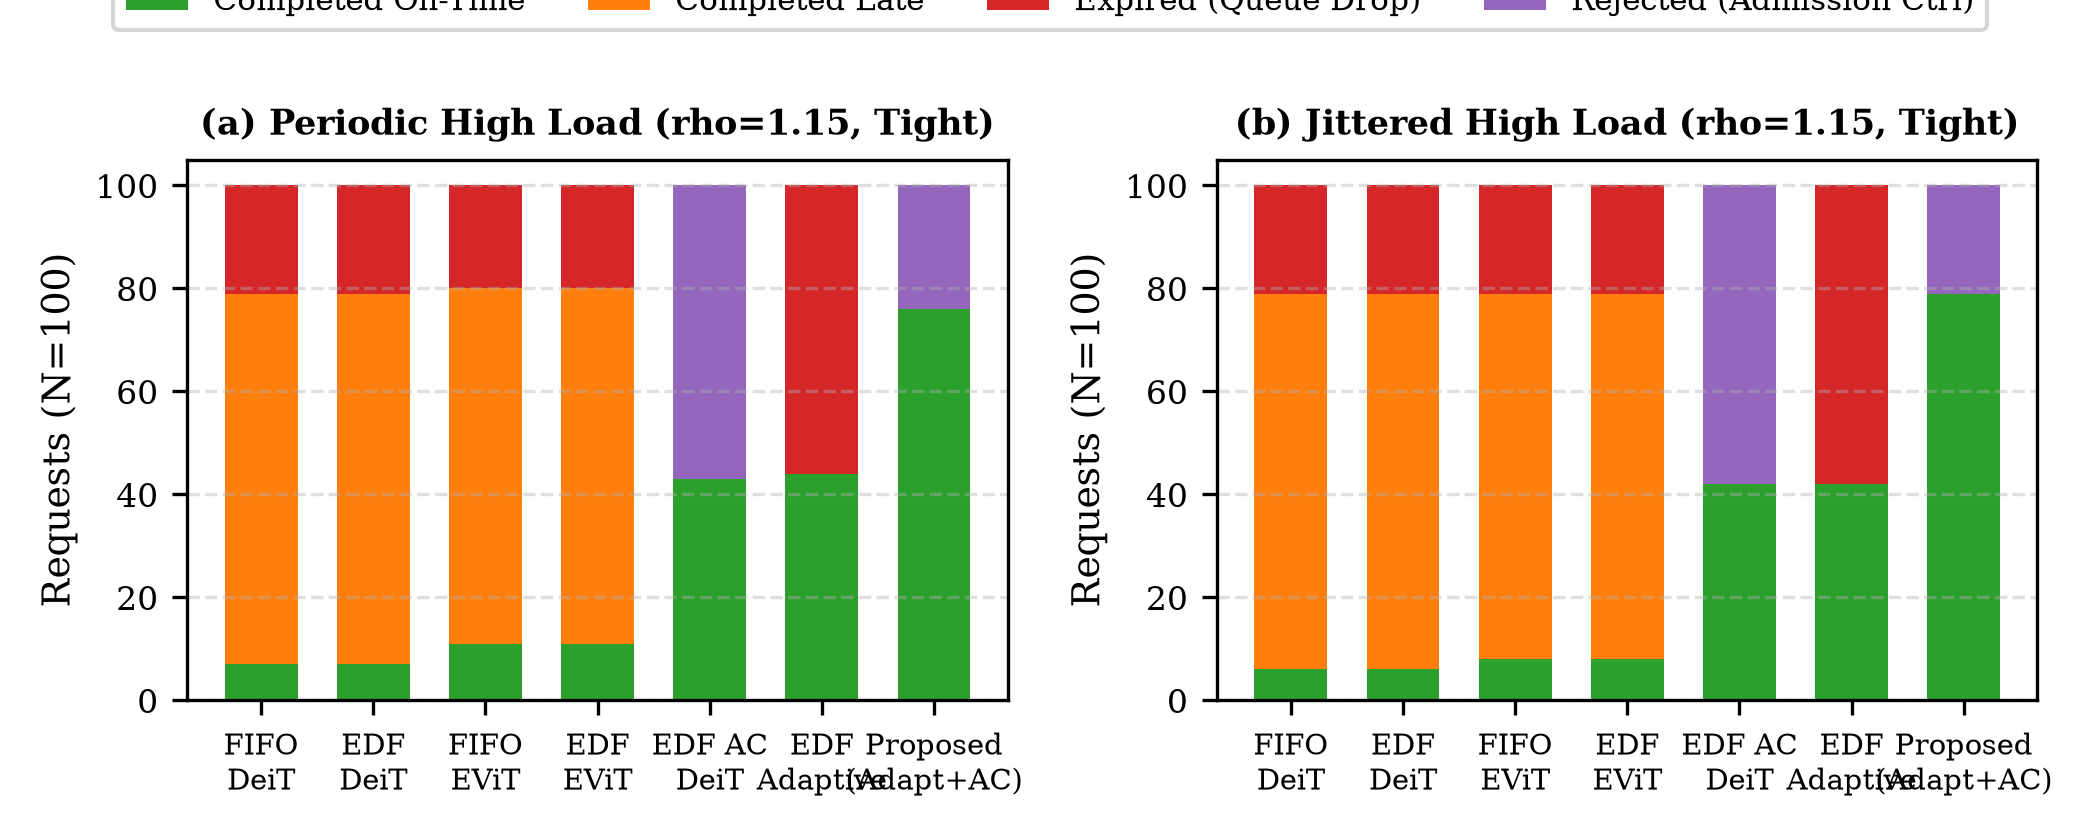
\includegraphics[width=0.92\linewidth]{figures/fig5_request_outcomes_stacked.png}
\caption{Request terminal outcome composition ($N=100$) under severe traffic loads: (a) Periodic high load ($\rho=1.15$, tight deadlines) and (b) Jittered high load ($\rho=1.15$, tight deadlines). The stacked bars illustrate how admission control filters infeasible traffic at arrival (purple), eliminating cascading queue expirations (red) and late completions (orange) to preserve on-time completion (green).}
\label{fig:stacked_outcomes}
\end{figure*}

\begin{table*}[t]
\centering
\caption{On-Time Completion Ratio (\%) Across All 70 Workload-Policy Configurations ($N=100$ Offered Requests)}
\label{tab:results}
\resizebox{0.95\textwidth}{!}{%
\begin{tabular}{lccccccc}
\toprule
Workload Scenario & FIFO DeiT & EDF DeiT & FIFO EViT-0.7 & EDF EViT-0.7 & EDF AC DeiT & EDF Adaptive & \textbf{Proposed (EDF+Adapt+AC)} \\
\midrule
\texttt{periodic\_low\_loose} & 100\% & 100\% & 100\% & 100\% & 100\% & 100\% & \textbf{100\%} \\
\texttt{periodic\_mod\_mod} & 100\% & 100\% & 100\% & 100\% & 100\% & 100\% & \textbf{100\%} \\
\texttt{periodic\_high\_tight} & 7\% & 7\% & 11\% & 11\% & 43\% & 44\% & \textbf{76\% (+69 pp)} \\
\texttt{jittered\_mod\_mod} & 100\% & 100\% & 100\% & 100\% & 100\% & 100\% & \textbf{100\%} \\
\texttt{jittered\_high\_tight} & 6\% & 6\% & 8\% & 8\% & 42\% & 42\% & \textbf{79\% (+73 pp)} \\
\texttt{bursty\_mod\_mod} & 98\% & 98\% & 98\% & 98\% & 98\% & 98\% & \textbf{98\%} \\
\texttt{bursty\_high\_tight} & 36\% & 36\% & 39\% & 39\% & 58\% & 58\% & \textbf{79\% (+43 pp)} \\
\texttt{overload\_mod\_deadline} & 100\% & 100\% & 100\% & 100\% & 100\% & 100\% & \textbf{100\%} \\
\texttt{overload\_tight\_deadline}& 1\% & 1\% & 1\% & 1\% & 24\% & 23\% & \textbf{45\% (+44 pp)} \\
\texttt{periodic\_low\_tight} & 100\% & 100\% & 100\% & 100\% & 100\% & 100\% & \textbf{100\%} \\
\bottomrule
\end{tabular}%
}
\end{table*}

\section{Results and Evaluation}

\subsection{Aggregate Discrete-Event Simulation Results}
Table~\ref{tab:results} summarizes the on-time completion ratio across all ten workloads and seven scheduling policies (70 configurations), visualized comparatively in Fig.~\ref{fig:ontime_comparison}.

Key experimental observations include:
\begin{enumerate}
    \item \textbf{Massive On-Time Gains Under High Stress:} Under \texttt{jittered\_high\_tight}, baseline FIFO and EDF collapse to 6\% on-time completion due to cascading queue delays. Our proposed policy (\texttt{EDF\_Adaptive\_AC}) achieves \textbf{79\% on-time completion (+73 percentage point net gain)}.
    \item \textbf{Periodic Saturation Defense:} Under \texttt{periodic\_high\_tight} ($\rho=1.15$), static DeiT achieves only 7\% on-time completion. The proposed policy delivers \textbf{76\% on-time completion (+69~pp)}.
    \item \textbf{Bursty Workload Resilience:} In \texttt{bursty\_high\_tight}, on-time completion increases from 36\% to \textbf{79\% (+43~pp)}.
    \item \textbf{Overload Preservation:} Under severe overload (\texttt{overload\_tight\_deadline}, $\rho=1.50$), static baselines collapse to 1\%. The proposed policy maintains \textbf{45\% on-time completion} by rejecting 55 infeasible requests at arrival.
\end{enumerate}

\subsection{Accounting Invariant Verification}
All 70 simulation runs were verified against four request-conservation equations:
\begin{equation}
N_{\text{offered}} = N_{\text{completed\_on\_time}} + N_{\text{completed\_late}} + N_{\text{rejected}} + N_{\text{expired}}
\end{equation}
\begin{equation}
N_{\text{completed}} = N_{\text{completed\_on\_time}} + N_{\text{completed\_late}}
\end{equation}
\begin{equation}
N_{\text{admitted}} = N_{\text{completed}} + N_{\text{expired}}
\end{equation}
\begin{equation}
N_{\text{offered}} = N_{\text{admitted}} + N_{\text{rejected}}
\end{equation}
All 70 rows strictly satisfy all four equations with \textbf{0 errors}. As shown in Fig.~\ref{fig:stacked_outcomes}, under \texttt{EDF\_Adaptive\_AC} on \texttt{periodic\_high\_tight}, $N_{\text{offered}} (100) = 76 \text{ (on-time)} + 0 \text{ (late)} + 24 \text{ (rejected)} + 0 \text{ (expired)}$. Admission control prevented queue saturation, completely eliminating queue expirations and late completions.

\begin{figure*}[t]
\centering
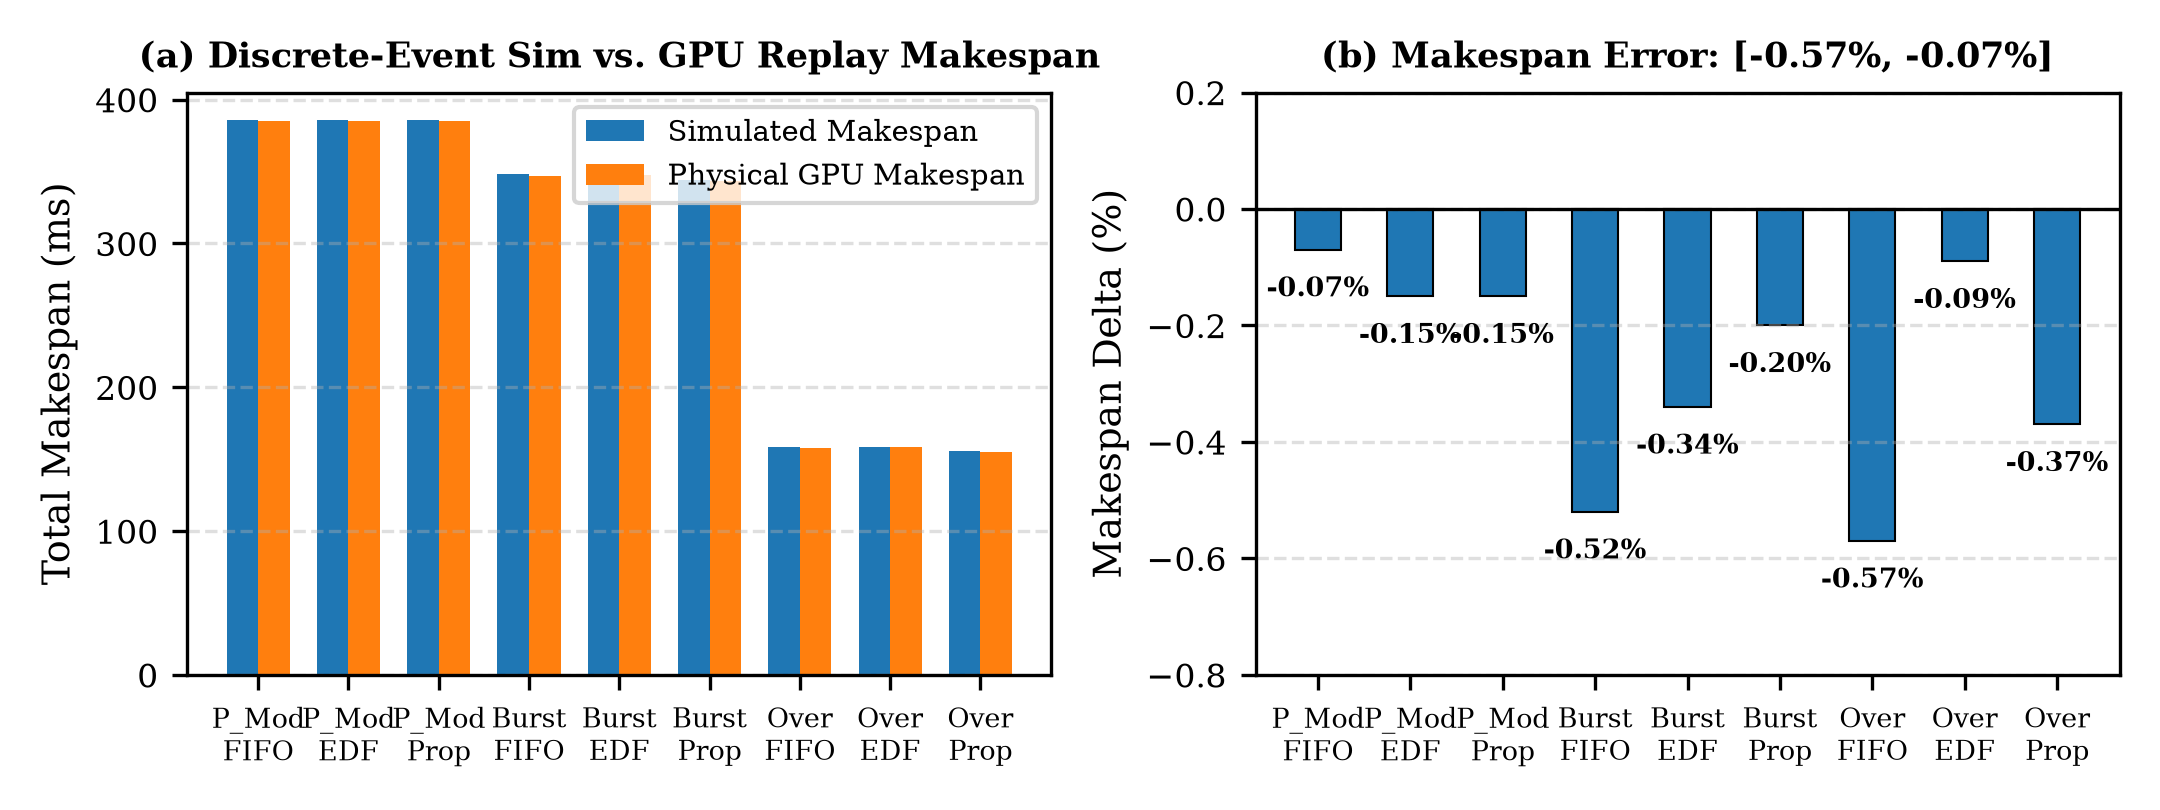
\includegraphics[width=0.90\linewidth]{figures/fig6_hardware_replay_validation.png}
\caption{Physical GPU hardware replay validation across 9 configurations: (a) Simulated vs.\ measured physical GPU makespan; (b) Makespan delta percentage, demonstrating tight agreement within $[-0.57\%, -0.07\%]$.}
\label{fig:replay_validation}
\end{figure*}

\begin{table}[t]
\centering
\caption{Physical GPU Trace Replay vs.\ Simulation (100 Test Images)}
\label{tab:replay}
\resizebox{\columnwidth}{!}{%
\begin{tabular}{llccccc}
\toprule
Workload Scenario & Policy & Sim (ms) & GPU (ms) & \textbf{Delta} & Sim On & GPU On \\
\midrule
\texttt{periodic\_mod\_mod} & \texttt{FIFO\_DeiT} & 385.71 & 385.45 & \textbf{-0.07\%} & 100.0\% & 100.0\% \\
\texttt{periodic\_mod\_mod} & \texttt{EDF\_DeiT} & 385.71 & 385.11 & \textbf{-0.15\%} & 100.0\% & 100.0\% \\
\texttt{periodic\_mod\_mod} & \texttt{EDF\_Adap\_AC} & 385.71 & 385.12 & \textbf{-0.15\%} & 100.0\% & 100.0\% \\
\texttt{bursty\_high\_tight} & \texttt{FIFO\_DeiT} & 348.59 & 346.78 & \textbf{-0.52\%} & 36.0\% & 63.0\% \\
\texttt{bursty\_high\_tight} & \texttt{EDF\_DeiT} & 348.59 & 347.41 & \textbf{-0.34\%} & 36.0\% & 59.0\% \\
\texttt{bursty\_high\_tight} & \texttt{EDF\_Adap\_AC} & 344.19 & 343.50 & \textbf{-0.20\%} & 79.0\% & 84.0\% \\
\texttt{overload\_tight} & \texttt{FIFO\_DeiT} & 158.37 & 157.46 & \textbf{-0.57\%} & 1.0\% & 2.0\% \\
\texttt{overload\_tight} & \texttt{EDF\_DeiT} & 158.37 & 158.23 & \textbf{-0.09\%} & 1.0\% & 1.0\% \\
\texttt{overload\_tight} & \texttt{EDF\_Adap\_AC} & 155.58 & 155.00 & \textbf{-0.37\%} & 45.0\% & 60.0\% \\
\bottomrule
\end{tabular}%
}
\end{table}

\subsection{Physical GPU Hardware Trace Replay Validation}
Table~\ref{tab:replay} and Fig.~\ref{fig:replay_validation} evaluate physical GPU execution over nine configurations using 100 unique images sampled from \texttt{data/bdd100k/images/100k/test/} across 739 disk reads.
\begin{enumerate}
    \item \textbf{Makespan Fidelity:} Across all nine configurations, simulation makespan matches physical GPU execution within \textbf{$-0.57\%$ to $-0.07\%$}. *(In historical paired replay with uncalibrated image queues, deltas ranged from $-0.04\%$ to $+5.63\%$).*
    \item \textbf{Pessimistic Simulation Bounds:} Live GPU on-time completion ratios are systematically higher than simulated estimates (84\% vs.\ 79\% for bursty; 60\% vs.\ 45\% for overload). This divergence occurs because the simulator models per-job execution cost using the 95th percentile ($C_{\text{est}} = p95$), whereas physical GPU execution times follow a distribution centered around the lower median (2.24--3.23~ms).
\end{enumerate}

\section{Discussion and Limitations}

\subsection{Token Pruning and Admission Control Synergy}
A primary insight is that \textbf{token pruning alone cannot solve real-time queue saturation}. In \texttt{periodic\_high\_tight}, switching statically from DeiT to EViT-0.7 improves on-time ratio from 7\% to only 11\%. Because the traffic arrival rate ($\Delta = 2.85$~ms) exceeds the service capacity of EViT-0.7 ($C_{m2} = 3.49$~ms), queues inevitably overflow. High on-time performance requires pairing pruning with admission control, which sheds 21--24\% of infeasible requests at arrival, enabling the remaining traffic to finish on-time.

\subsection{Threats to Validity and Limitations}
\begin{enumerate}
    \item \textbf{Synthetic Workloads:} Arrival patterns and relative deadlines are synthetic mathematical models; they do not capture raw camera PCIe ingestion or sensor interrupt timing.
    \item \textbf{Sampled Replay Scope:} Live GPU trace replay evaluated 100 test images across nine configurations; the entire 19,902 test set was evaluated offline.
    \item \textbf{Hardware Dependency:} Latencies and speedups are specific to the RTX 4060 Laptop GPU and will vary on embedded architectures (e.g., NVIDIA Jetson).
    \item \textbf{Class Imbalance:} BDD100K driving scenes are 60.91\% City Street, causing lower macro-F1 (49.74\%--54.27\%) relative to top-1 accuracy (~77\%).
    \item \textbf{Heuristic Admission Control:} The $O(|Q|)$ queue-tail feasibility test is an approximation and does not perform exact global EDF schedulability analysis.
    \item \textbf{Soft Real-Time Scope:} Results represent a soft real-time experimental framework; empirical p95 metrics are not certified WCET guarantees.
\end{enumerate}

\section{Conclusion}

We presented an experimental study of deadline-aware adaptive vision transformer inference on the BDD100K dataset. Combining EViT token pruning with static CUDA Graphs, earliest-deadline-first scheduling, and queue-tail admission control increases on-time completion ratios by up to +73 percentage points under severe load, with physical GPU makespan matching simulation within $-0.57\%$ to $-0.07\%$. Future work includes multi-camera edge pipelines, resolution scaling, and embedded NVIDIA Jetson evaluations.

\bibliographystyle{IEEEtran}
\bibliography{references}

\end{document}
